\documentclass[12pt,letterpaper,noanswers]{exam}
\usepackage[usenames,dvipsnames,svgnames,table]{xcolor}
\usepackage[margin=0.9in]{geometry}
\renewcommand{\familydefault}{\sfdefault}
\usepackage{multicol}
\pagestyle{head}
\header{AM 111 Class 11}{}{Piecewise interpolation, p.\thepage}
\runningheadrule
\headrule
\usepackage{siunitx}
\usepackage{graphicx} % more modern
\usepackage{amsmath} 
\usepackage{amssymb} 
\usepackage{hyperref}
\usepackage{tcolorbox}
\usepackage{enumitem}
\def\mbf{\mathbf}
\newcommand{\vc}[1]{\boldsymbol{#1}}
\def\dsst{\displaystyle}
\DeclareMathOperator*{\argmin}{arg\,min} % thin space, limits underneath in displays


\begin{document}
 \pdfpageheight 11in 
  \pdfpagewidth 8.5in

\noindent 

\section*{Preliminaries}

\begin{itemize}
\itemsep0pt
\item The quiz is Thursday.
\end{itemize}



\noindent\textbf{Big picture}

Today: Algorithms for finding a piecewise polynomial that directly passes through data points.

\vspace{0.2cm}
\hrule
\vspace{0.2cm}

\noindent \textbf{Skill check practice}

Does the following form a cubic spline interpolating $(1,2), (2,1), (4,4)$?

$S_1(x) = 2- \frac{13}{8}(x-1) + \frac{5}{8}(x-1)^3$ on $[1,2]$

$S_2(x) = 1 + \frac{1}{4}(x-2) + \frac{15}{8}(x-2)^2 - \frac{5}{8}(x-2)^3$ on $[2,4]$.



% Set up the matrix equation to find the natural cubic spline through $(0,3), (1,-2), (2,1), (3,3)$ where the system of equations is given by

% $\delta_1 c_1 + 2(\delta_1+\delta_2)c_2 + \delta_2c_3 = 3\left(\dfrac{\Delta_2}{\delta_2} - \dfrac{\Delta_1}{\delta_1}\right)$

% $\delta_2 c_2 + 2(\delta_2+\delta_3)c_3 + \delta_3 c_4= 3\left(\dfrac{\Delta_3}{\delta_3} - \dfrac{\Delta_2}{\delta_2}\right)$

% $2c_1 = 0$

% $2c_4 = 0$

% where $\delta_k = x_{k+1} - x_k$ and $\Delta_k = y_{k+1}-y_k$.

\vspace{0.2cm}
\hrule
\vspace{0.2cm}

\noindent \textbf{Skill check solution}

1) Check $S_k(x_{k+1}) = y_{k+1}$.  

$S_1(2) = 2 - 13/8 + 5/8 = 2 - 1 = 1$

$S_2(4) = 1 + 1/2 + 15/2 - 5 = 1+8-5 = 4$

Passes this check

2) Check $S'$ is continuous.

$S'_1 = -\frac{13}{8} + 3\frac{5}{8}(x-1)^2$.  $S'_1(2) = -\frac{13}{8}+\frac{15}{8} = \frac{1}{4}$

$S'_2 = \frac{1}{4} + \frac{15}{4}(x-2) - \frac{15}{8}(x-2)^2$.  $S'_2(2) = \frac{1}{4} $

Passes this check.

3) Check $S''$ is continuous

$S''_1 =  3\frac{5}{4}(x-1)$.  $S''_1(2) = \frac{15}{4}$

$S''_2 = \frac{15}{4} - \frac{15}{4}(x-2)$.  $S''_2(2) = \frac{15}{4} $

Passes this check.

$\left\{S_1, S_2\right\}$ forms a cubic spline interpolating the points.

% Creating the matrix equation, use $\left[\begin{array}{c} c_1 \\ c_2 \\ c_3 \\ c_4 \end{array}\right]$ for the vector of unknown coefficients.

% Put $c_1 = 0$ in the first row and $c_4 = 0$ in the 4th row.

% The $\delta_k = 1$.  $\Delta_1 = -2-3 = -5$, $\Delta_2= 1--2 = 3$, $\Delta_3 = 3-1 = 2.$

% $\Delta_2/1 - \Delta_1/1 = 3--5 = 8$.  $\Delta_3/1 - \Delta_2/1 = 2-3 = -1$

% The matrix equation is $\left[\begin{array}{c c c c}1 & 0 & 0 & 0 \\
% 1 & 4 & 1 & 0 \\
% 0 & 1 & 4 & 1 \\
% 0 & 0 & 0 & 1\end{array}\right]\left[\begin{array}{c} c_1 \\ c_2 \\ c_3 \\ c_4 \end{array}\right] = \left[\begin{array}{c} 0 \\ 24 \\ -3 \\ 0\end{array}\right]$

\vspace{0.2cm}
\hrule
\vspace{0.2cm}



\section*{Piecewise polynomial interpolation (splines)}

(Koumoutsakos et al lecture 4, Sauer \S 3.4)


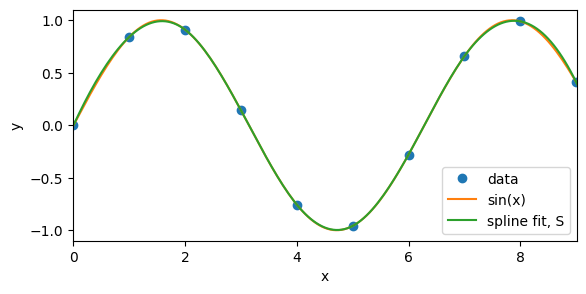
\includegraphics[width=0.5\textwidth]{img/Class09sinspline.png}
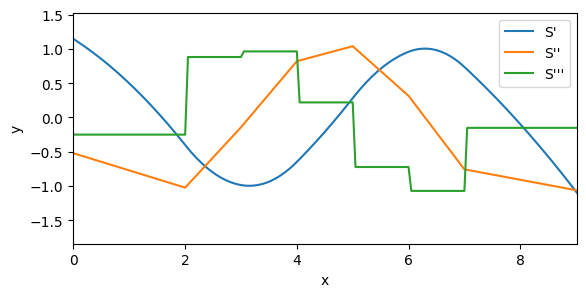
\includegraphics[width=0.5\textwidth]{img/Class09deriv.png}

\begin{enumerate}[resume]
\item $\sin x$ is shown above with a spline fit, $S$, where $S$ is a piecewise polynomial of degree $n$.  On the right are plotted $S', S'',S'''$.  



The spline fit, $S(x) = \left\{\begin{array}{l l} S_1(x) & x_0\leq x < x_1 \\
S_2(x) & x_1\leq x < x_2 \\
\vdots \\
S_k(x) & x_{k-1}\leq x < x_k \\
\end{array}\right.$
\begin{parts}
\item Using the graphs, identify the degree of $S_j(x)$.
\vspace{1cm}

\item Using the graphs, find $k$ (the total number of pieces for the piecewise function).

\vspace{1cm}

\item Is $S$ a continuous function?  Is it differentiable?  How do you know?

\emph{This question is about $S$, and not about its components $S_j$.}
\vspace{1cm}

\end{parts}
\end{enumerate}

\subsection*{Cubic splines}

\begin{enumerate}[resume]
\item 
\begin{parts}
\item How many unknowns are there in the definition of $S(x)$?
\vspace{1cm}

\item How many constraints arise from imposing $S(x_i) = y_i$ and $S_i(x_{i+1}) = y_{i+1}$?


\vspace{1cm}

\item How many more constraints are needed to uniquely identify the unknowns?
\vspace{1cm}

\item How many additional constraints come from continuity of the first derivative and continuity of the second derivative?  How many more are needed?
\vspace{1cm}

\end{parts}
\end{enumerate}

\noindent\textbf{Final parameters}


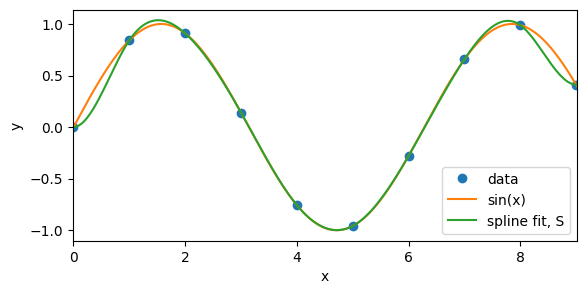
\includegraphics[width=0.5\textwidth]{img/Class09clamp.png}
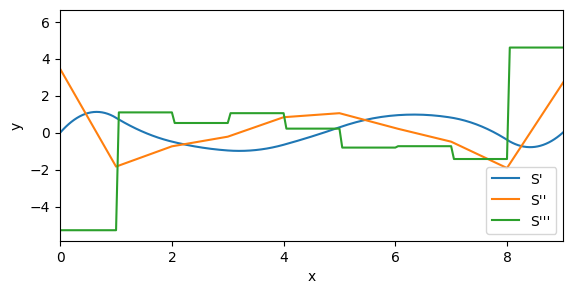
\includegraphics[width=0.5\textwidth]{img/Class09clampderiv.png}

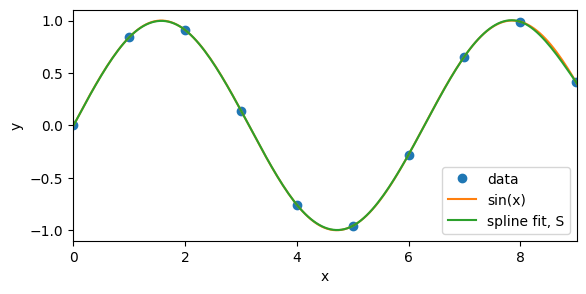
\includegraphics[width=0.5\textwidth]{img/Class09natural.png}
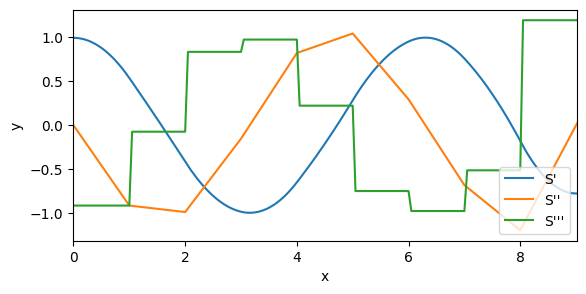
\includegraphics[width=0.5\textwidth]{img/Class09naturalderiv.png}

\begin{enumerate}[resume]
    \item Three different spline fits to $\sin x$ are given (call them A: p.1, B: top of the pair, C: 2nd in the pair)  Match each of them to one of the ways of setting additional constraints.
    
    \emph{How did you make your matches?}
    
    \vspace{1cm}
    
    \item Provide the constraint equations associated with ``not-a-knot''.
\vspace{1in}
    
\end{enumerate}

\subsection*{Finding coefficients}

\subsection*{Natural spline}

Each of the three properties generates equations.
\begin{enumerate}[resume]
\item Denote $x_{i+1}-x_i = \delta_i$ and $y_{i+1}-y_i$ as $\Delta_i$.  

Use $S''_{i-1}(x_i) = S''_i(x_i)$ and $S_i(x) = y_i + b_i(x-x_i) + c_i(x-x_i)^2 + d_i(x-x_i)^3$ to write $d_{i}$ in terms of $c_{i+1}$, $c_i$, and $\delta_i$.

\vspace{1in}

%\emph{For convenience introduce an extra unknown, $c_n = S''_{n-1}(x_n)/2$.}

\end{enumerate}


\begin{enumerate}[resume]
\item Find the natural cubic spline through $(0,4), (1,-1), (2,2)$.  Treat $c_1, c_2, c_3$ as the three unknowns.

Two equations come from the boundary conditions for natural cubic splines:

$S_1''(x_1) = 0 \Rightarrow 2c_1 = 0$.

$S_3''(x_3) = 0 \Rightarrow 2c_3 = 0$.

The third equation is

$\delta_k c_k + 2(\delta_k+\delta_{k+1})c_{k+1} + \delta_{k+1}c_{k+2} =3 \left(\dfrac{\Delta_{k+1}}{\delta_{k+1}} - \dfrac{\Delta_k}{\delta_k}\right)$

with $k = 1$.

Set up a matrix equation with a vector of unknowns $\left[\begin{array}{c} c_1 \\ c_2 \\ c_3 \end{array}\right]$.

\vspace{1in}

\item Solve your matrix equation.
\vspace{1in}

\item There are four other boundary conditions we might consider (recall that our spline, $S$, consists of $n-1$ segments, $S_1, S_2, ..., S_{n-1}$):
\begin{itemize}
 \item ``not-a-knot'': 1st two segments ($S_1$ and $S_2$) and last two ($S_{n-2}$ and $S_{n-1}$) have the same cubic
    \item parabolic runout: set $S_1''(x_1) = S_1''(x_2)$ and $S_n''(x_n) = S_n''(x_{n-1})$
    \item clamping: set $S_1'(x_1) = S_{n-1}'(x_n) = 0$
    \item periodic: set $S_1'(x_1) = S_{n-1}'(x_n)$ and $S_1''(x_1) = S_{n-1}''(x_n)$
\end{itemize}
Choose one of these and adjust your matrix equation to reflect it.

\vspace{1in}
\end{enumerate}









\begin{enumerate}[resume]
\item Consider the system \[\left[\begin{array}{c c c c}
1 & 2 & 0 & 0 \\
2 & 3 & 4 & 0 \\
0 & 1 & 7 & 3\\
0 & 0 & 4 & 2
\end{array}\right]\vc{x} = \left[\begin{array}{c} 
1 \\ 6 \\ 7 \\ 2
\end{array}\right]\]

\begin{parts}
\item Eliminate the $a_i$ elements.  Divide the first row by $b_1$, multiply by $a_2$, and subtract if from the second row.  Continue with this procedure to create an upper triangular matrix.
\vfill

\item How many addition, subtraction, multiplication, division operations did this require?  These are basic floating point operations, FLOPs.
\vspace{1cm}

\item Use back substitution to solve your resulting matrix.
\vfill

\item Again count the FLOPs.

\end{parts}

This algorithm for solving a tridiagonal system is $\mathcal{O}(N)$.
\end{enumerate}


\href{https://edsonmarine.com/set-of-six-bronze-spline-weights/}{Splines for sale}
\end{document}